\tikzstyle{node}=[
  draw,
  circle,
  very thick,
  color=black,
  fill=white,
]%
%
\tikzstyle{node_filled}=[
  draw,
  circle,
  very thick,
  color=black,
  fill=orange!50!yellow
]%
%
\tikzstyle{node_leaf}=[
  draw,
  circle,
  very thick,
  color=black,
  fill=green!50!white,
]%
%
\tikzstyle{path}=[
  draw,
  line width=0.25em,
  color=orange!50!yellow!80!black
]%
%
\tikzstyle{path_normal}=[
  draw,
  very thick,
  color=black
]%
%
\begin{adjustbox}{width=\linewidth}
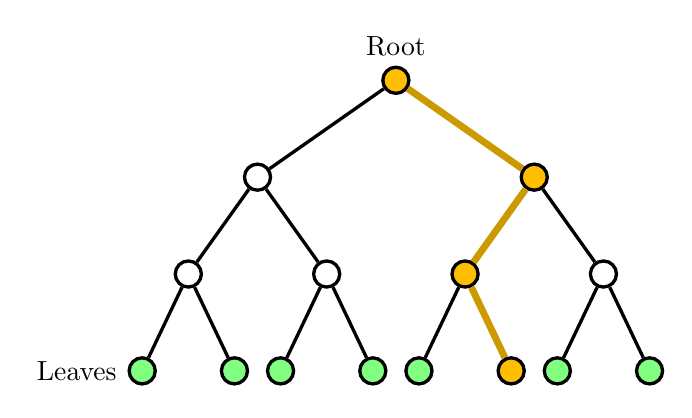
\begin{tikzpicture}[
  level/.style={
    sibling distance = 10.0em/#1,
    level distance = 3.5em
  }
]
\node [node_filled, label={[anchor=south]above:Root}] (root) {}
child [path_normal] {
  node [node] {}
  child {
    node [node] {}
    child {node [node_leaf, label={[anchor=east]left:Leaves}] {}}
    child {node [node_leaf] {}}
  }
  child {
    node [node] {}
    child {node [node_leaf] {}}
    child {node [node_leaf] {}}
  }
}
child [path] {
  node [node_filled] {}
  child {
    node [node_filled] {}
    child [path_normal] {node [node_leaf] {}}
    child {node [node_filled] {}}
  }
  child [path_normal] {
    node [node] {}
    child {node [node_leaf] {}}
    child {node [node_leaf] {}}
  }
};
\end{tikzpicture}
\end{adjustbox}